\begin{figure}
  \centering
  \tikzstyle{base}=[rectangle,
                    draw=black,
                    minimum width=4cm,
                    minimum height=1cm,
                    text centered]
  \definecolor{FixedColor}{rgb}{1.0,0.901,0.805}
  \definecolor{ProgrammableColor}{rgb}{0.7,0.9,1.0}
                           
  \tikzstyle{programmable}=[base, fill={ProgrammableColor}]
  \tikzstyle{fixed}=[base, fill={FixedColor}]
  \tikzstyle{optional}=[rounded corners]
  
  \begin{subfigure}{.48\textwidth}
    \centering
    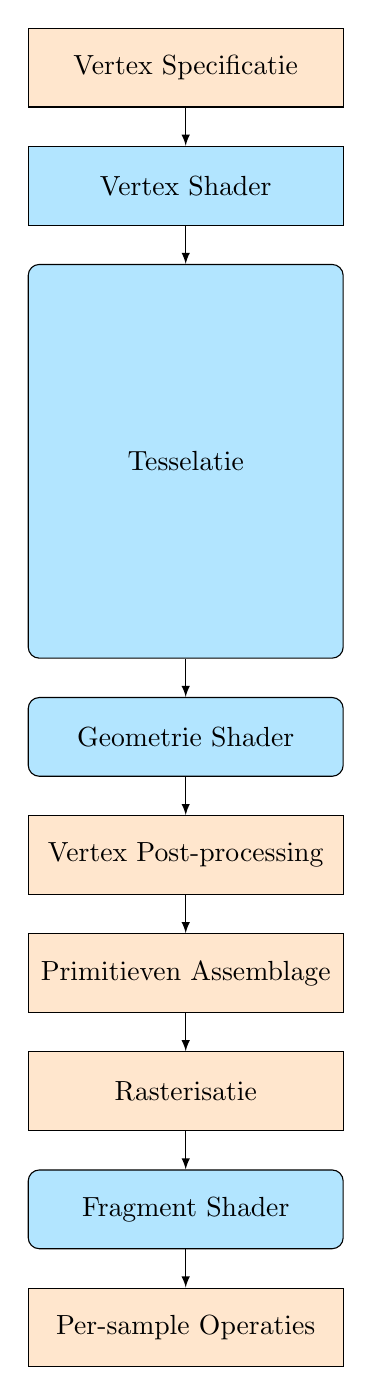
\begin{tikzpicture}[node distance=1.5cm
                        every node/.style={fill=white},
                        align=center]
    
      \node at (0.0,   0.0) (vertex_spec)   [fixed]                                      {Vertex Specificatie};
      \node at (0.0,  -1.5) (vertex_shader) [programmable]                               {Vertex Shader};
      \node at (0.0,  -5.0) (tess_shader)   [programmable, optional, minimum height=5cm] {Tesselatie};
      \node at (0.0,  -8.5) (geom_shader)   [programmable, optional]                     {Geometrie Shader};
      \node at (0.0, -10.0) (vertex_post)   [fixed]                                      {Vertex Post-processing};
      \node at (0.0, -11.5) (prim_ass)      [fixed]                                      {Primitieven Assemblage};
      \node at (0.0, -13.0) (rasterisation) [fixed]                                      {Rasterisatie};
      \node at (0.0, -14.5) (frag_shader)   [programmable, optional]                     {Fragment Shader};
      \node at (0.0, -16.0) (per_sample)    [fixed]                                      {Per-sample Operaties};
    
      \draw[-latex] (vertex_spec)   -- (vertex_shader);
      \draw[-latex] (vertex_shader) -- (tess_shader);
      \draw[-latex] (tess_shader)   -- (geom_shader);
      \draw[-latex] (geom_shader)   -- (vertex_post);
      \draw[-latex] (vertex_post)   -- (prim_ass);
      \draw[-latex] (prim_ass)      -- (rasterisation);
      \draw[-latex] (rasterisation) -- (frag_shader);
      \draw[-latex] (frag_shader)   -- (per_sample);
  \end{tikzpicture}
    \caption{openGL}\label{fig:mgp-pipeline-opengl}
  \end{subfigure}%
  \begin{subfigure}{.48\textwidth}
    \centering
    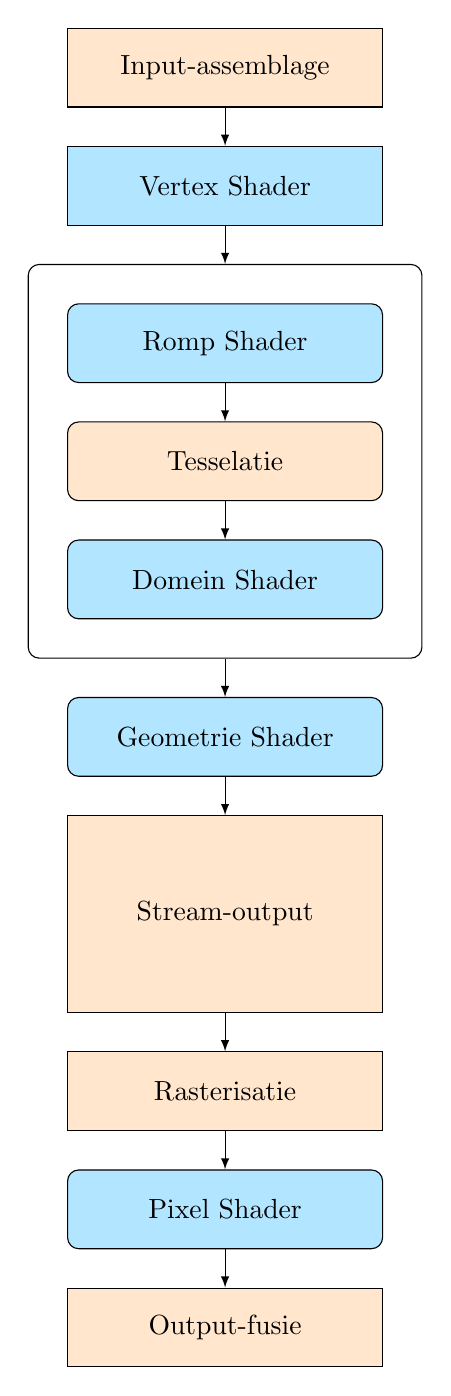
\begin{tikzpicture}[node distance=1.5cm
                        every node/.style={fill=white},
                        align=center]
    
    \node at (0.0,   0.00) (vertex_spec)      [fixed]                       {Input-assemblage};
    \node at (0.0,  -1.50) (vertex_shader)    [programmable]                {Vertex Shader};
    \node at (0.0,  -3.50) (hull_shader)      [programmable, optional]      {Romp Shader};
    \node at (0.0,  -5.00) (tesselation)      [fixed, optional]             {Tesselatie};
    \node at (0.0,  -6.50) (domain_shader)    [programmable, optional]      {Domein Shader};
    \node at (0.0,  -5.00) (tesselation_comp) [rectangle, draw=black, minimum height=5cm, minimum width = 5cm, optional] {};    
    \node at (0.0,  -8.50) (geom_shader)      [programmable, optional]      {Geometrie Shader};
    \node at (0.0, -10.75) (prim_ass)         [fixed, minimum height=2.5cm] {Stream-output};
    \node at (0.0, -13.00) (rasterisation)    [fixed]                       {Rasterisatie};
    \node at (0.0, -14.50) (frag_shader)      [programmable, optional]      {Pixel Shader};
    \node at (0.0, -16.00) (per_sample)       [fixed]                       {Output-fusie};

    
     \draw[-latex] (vertex_spec)      -- (vertex_shader);
     \draw[-latex] (vertex_shader)    -- (tesselation_comp);
     \draw[-latex] (hull_shader)      -- (tesselation);
     \draw[-latex] (tesselation)      -- (domain_shader);
     \draw[-latex] (tesselation_comp) -- (geom_shader);
     \draw[-latex] (geom_shader)      -- (prim_ass);
     \draw[-latex] (prim_ass)         -- (rasterisation);
     \draw[-latex] (rasterisation)    -- (frag_shader);
     \draw[-latex] (frag_shader)      -- (per_sample);
  \end{tikzpicture}
    \caption{Direct3D}\label{fig:mgp-pipeline-direct3d}
  \end{subfigure}
  \caption{De stappen van zowel de openGL als Direct3D implementaties.}
  \label{fig:mgp-pipeline}
\end{figure}
